% Complete LaTeX manuscript prepared for Overleaf
% This version uses the standard article class to avoid missing Springer class errors.
% After the scientific text is stable, it can be migrated back to the Springer Nature sn-jnl template.

\documentclass[12pt,a4paper]{article}

\usepackage[utf8]{inputenc}
\usepackage[T1]{fontenc}
\usepackage{lmodern}
\usepackage{graphicx}
\usepackage{booktabs}
\usepackage{amsmath,amssymb}
\usepackage{array}
\usepackage{tabularx}
\usepackage{geometry}
\usepackage{setspace}
\usepackage{authblk}
\usepackage{url}
\usepackage[numbers,sort&compress]{natbib}
\usepackage[hidelinks]{hyperref}
\usepackage{caption}
\usepackage{float}
\usepackage{placeins}
\usepackage{microtype}

\hypersetup{
  pdfauthor={},
  pdfcreator={},
  pdfproducer={},
  pdfsubject={},
  pdfkeywords={}
}

\geometry{margin=2.5cm}
\onehalfspacing
\setlength{\emergencystretch}{3em}
\newcolumntype{Y}{>{\raggedright\arraybackslash}X}
\providecommand{\bibcommenthead}{}

\title{An Intelligent Behavioral Monitoring Platform for Observational Learning Analytics in Basic Education}

\author{}

\date{}

\begin{document}

\maketitle

\begin{abstract}
Contemporary educational environments increasingly demand technological approaches capable of supporting teachers in monitoring classroom engagement and behavioral interaction patterns. In this context, Artificial Intelligence in Education, Learning Analytics, and Computer Vision have emerged as promising interdisciplinary fields for the development of intelligent educational support systems. This study presents an intelligent behavioral monitoring platform designed to support observational learning analytics in basic education through real-time computer vision and temporal behavioral analysis. The proposed platform integrates YOLOv11-Pose \cite{zhuCsbyoloRapidEfficient2024} for human pose estimation, InsightFace with ArcFace embeddings for facial recognition, and PostgreSQL combined with PGVector for vector similarity search and embedding storage. Behavioral interpretation is performed through geometric analysis of body keypoints extracted from classroom video streams captured in a controlled experimental environment using RTSP cameras. Rather than attempting emotional inference or psychological diagnosis, the system focuses on observable classroom behavioral patterns associated with attentive behavior, distraction tendencies, agitation, prolonged downward posture, and questioning-related gestures. The results demonstrate the feasibility of integrating Computer Vision and Learning Analytics into a unified educational platform capable of supporting pedagogical reflection while preserving ethical and privacy considerations through embedding-based facial representation and restricted educational usage.
\end{abstract}

\noindent\textbf{Keywords:} Artificial Intelligence in Education; Learning Analytics; Computer Vision; Behavioral Monitoring; Intelligent Educational Systems; Educational Technology.

\section{Introduction}

Educational environments have progressively become more complex due to increasing classroom heterogeneity, prolonged instructional demands, and the growing necessity for individualized pedagogical observation. In face-to-face educational contexts, teachers are frequently required to conduct instructional activities, manage classroom organization, observe student participation, and identify engagement tendencies under limited temporal and cognitive conditions \cite{trabelsiRealTimeAttentionMonitoring2023a,yuvarajAutomatedRecognitionTeacher2024,zhangSmartClassroomsHow2024}.

Within this scenario, Artificial Intelligence in Education and Learning Analytics have emerged as relevant interdisciplinary research fields capable of supporting educational observation and pedagogical decision-making through computational analysis of educational data \cite{zhangSmartClassroomsHow2024,zhangAreThereFundamental2024}. Existing studies have demonstrated the potential of intelligent systems to assist teachers in understanding learning dynamics, interaction patterns, and student engagement tendencies \cite{chenStudentBehaviorDetection2023,huRealTimeClassroomBehavior2024}.

Most Learning Analytics approaches traditionally rely on data extracted from virtual learning environments, online educational systems, or academic performance indicators \cite{araComprehensiveSurveyLearning2023}. Comparatively fewer studies investigate observational classroom analytics based on real-time behavioral monitoring in physical educational environments. This limitation is particularly relevant in basic education, where classroom observation remains strongly dependent on the teacher's perception and accumulated professional experience.

Recent advances in Computer Vision and Deep Learning have enabled the application of pose estimation, facial recognition, and activity analysis techniques within educational contexts \cite{liangYOLObasedBehaviorDetection2025,liRealTimeClassroomBehavior2025}. Nevertheless, many existing approaches remain strongly centered on technical performance metrics or affective inference models, often providing limited pedagogical interpretation and raising ethical concerns regarding emotional recognition and automated student profiling.

Considering these limitations, the present study proposes an intelligent behavioral monitoring platform designed to support observational learning analytics in classroom environments through Computer Vision and temporal behavioral interpretation. The proposed monitoring framework integrates YOLOv11-Pose for real-time human pose estimation, InsightFace with ArcFace embeddings for facial recognition \cite{dengArcFaceAdditiveAngular,anKillingTwoBirds2022,nRealTimeFace2023}, and PostgreSQL integrated with PGVector for vector similarity search and embedding management \cite{zhangAreThereFundamental2024,panSurveyVectorDatabase2024}.
% TODO AUTOR: inserir referência técnica oficial sobre YOLOv11-Pose.
% TODO AUTOR: inserir referência técnica oficial sobre PostgreSQL e PGVector, se a política editorial permitir documentação técnica.

Rather than attempting to infer emotional or psychological states, the proposed system focuses exclusively on observable classroom interaction patterns associated with pedagogical observation. The behavioral analysis module was designed to identify tendencies related to attentive posture, distraction patterns, agitation, prolonged downward head positioning, and hand-raising interactions commonly associated with questioning behavior.

One of the central contributions of the proposed framework involves temporal behavioral analytics capable of supporting reflective pedagogical observation over time instead of relying on isolated behavioral events. The system was therefore conceived as a teacher-support tool, not as a mechanism for clinical, psychological, or disciplinary diagnosis.

\section{Related work}


\subsection{Learning Analytics and Artificial Intelligence in Education}

Learning Analytics has emerged as an interdisciplinary research field focused on the collection, analysis, and interpretation of educational data to support pedagogical decision-making and improve learning processes \cite{araComprehensiveSurveyLearning2023,zhangSmartClassroomsHow2024}. Rather than emphasizing exclusively academic performance metrics, contemporary Learning Analytics approaches increasingly investigate classroom engagement, participation dynamics, and behavioral interaction patterns capable of supporting reflective educational practices \cite{huRealTimeClassroomBehavior2024,mitomaBehaviorMonitoringSystem2025}.

Artificial Intelligence in Education has progressively contributed to the development of intelligent educational support systems capable of assisting teachers in understanding instructional dynamics and classroom interaction tendencies \cite{zhangSmartClassroomsHow2024,huRealTimeClassroomBehavior2024}. Within this context, Computer Vision techniques have demonstrated significant potential for enabling observational classroom analytics through automated visual interpretation of engagement, participation, and classroom behavior indicators \cite{chenStudentBehaviorDetection2023,yuvarajAutomatedRecognitionTeacher2024,yangStudentClassroomBehavior2024}.

Recent educational research highlights the importance of intelligent systems that support teachers without replacing pedagogical autonomy, particularly because automated monitoring can raise concerns regarding privacy, interpretability, emotional inference, and excessive behavioral simplification \cite{trabelsiRealTimeAttentionMonitoring2023a,xiaoOcclusionRobustCognitive2024,zhangSmartClassroomsHow2024}. Consequently, explainable observational analytics and ethically oriented educational monitoring approaches have become increasingly relevant within educational technology research.

\subsection{Computer Vision Applications in Educational Environments}

Advances in Deep Learning and Computer Vision have enabled the application of intelligent monitoring systems in educational environments. Human pose estimation, activity recognition, facial detection, and classroom behavior analysis techniques have progressively expanded within Artificial Intelligence in Education research.

Pose estimation approaches based on convolutional neural networks allow the extraction of anatomical keypoints associated with body posture and movement dynamics \cite{zhuCsbyoloRapidEfficient2024}. These techniques enable the identification of behavioral tendencies associated with participation, distraction, movement, and classroom engagement.

For example, Yuvaraj et al. proposed a long-term recurrent convolutional network (LRCN) that combines convolutional feature extraction with recurrent temporal modeling to recognize teacher and student activities in classroom videos, including instructional and learner actions relevant to classroom observation \cite{yuvarajAutomatedRecognitionTeacher2024}. Similarly, Yang and Wang investigated spatio-temporal student classroom behavior detection and multi-model fusion for behaviors such as hand-raising, reading, and writing \cite{yangStudentClassroomBehavior2024}. These studies demonstrate the relevance of temporal visual modeling for educational behavior analysis, although they differ from the present work because the proposed platform emphasizes real-time observational indicators, facial association with registered students, and interpretable geometric criteria for teacher support.

\begin{figure}[!htbp]
\centering
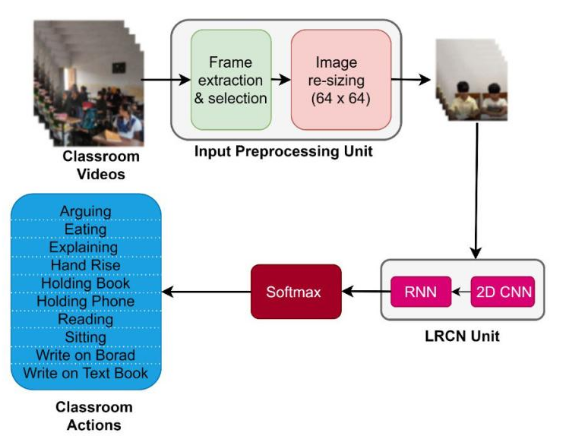
\includegraphics[width=0.70\textwidth]{cv_classroom_pipeline.png}
\caption{Example of a Computer Vision pipeline applied to classroom behavior recognition using convolutional and recurrent neural networks. Adapted from \cite{yuvarajAutomatedRecognitionTeacher2024}. Recent educational monitoring systems have progressively adopted hybrid Computer Vision architectures for classroom behavior interpretation \cite{chenStudentBehaviorDetection2023,huRealTimeClassroomBehavior2024}.}
\label{fig:cv_education}
\end{figure}

Among contemporary approaches, the YOLO family has demonstrated high performance in real-time object detection and pose estimation tasks \cite{liangYOLObasedBehaviorDetection2025,liRealTimeClassroomBehavior2025}. Such models have enabled efficient classroom monitoring scenarios involving multiple individuals simultaneously observed through video streams.

Despite these advances, studies such as Chen et al., Liang et al., Li et al., Sheng et al., and Zhang et al. primarily report detection-oriented outcomes using indicators such as precision, mAP, recall, model size, or latency, while their pedagogical discussion is generally secondary to the optimization of visual detection models \cite{chenStudentBehaviorDetection2023,liangYOLObasedBehaviorDetection2025,liRealTimeClassroomBehavior2025,shengRealtimeClassroomStudent2025,zhangClassroomBehaviorDetection2025}. Other works move beyond observable behavior detection toward attention, cognitive engagement, or emotional-state inference; for instance, Trabelsi et al. monitor attention and emotional states, Xiao et al. detect cognitive engagement, and Hossen and Uddin classify attention in online classes \cite{trabelsiRealTimeAttentionMonitoring2023a,xiaoOcclusionRobustCognitive2024,hossenAttentionMonitoringStudents2023}. This distinction is important because detecting visible behaviors such as hand-raising or head orientation is not equivalent to inferring engagement, emotion, or psychological condition. The present study therefore adopts a more restricted observational scope: it uses interpretable geometric criteria to support teacher reflection without performing emotional recognition, psychological profiling, or automated diagnostic classification.

Considering these limitations, the present study adopts an observational perspective focused on interpretable classroom interaction patterns rather than emotional or psychological inference.

\subsection{Facial Recognition and Embedding-Based Educational Monitoring}
Facial recognition systems based on deep neural networks have progressively evolved through the use of embedding-based representations capable of converting facial characteristics into multidimensional numerical vectors optimized for similarity comparison \cite{schroffFaceNetUnifiedEmbedding2015,dengArcFaceAdditiveAngular}.

Among contemporary approaches, ArcFace has demonstrated high discriminative performance through additive angular margin optimization, enabling robust facial embedding generation suitable for identification tasks in real-time environments \cite{dengArcFaceAdditiveAngular}. InsightFace-related research and implementations integrate facial detection, alignment, and embedding extraction within unified facial analysis pipelines \cite{dengRetinaFaceSinglestageDense2019,anKillingTwoBirds2022,nRealTimeFace2023}.

ArcFace-based facial recognition architectures operate through embedding representations projected into normalized hyperspherical vector spaces. In this approach, facial identities are represented as multidimensional numerical vectors optimized for angular discrimination through additive margin learning \cite{dengArcFaceAdditiveAngular}. Consequently, cosine similarity becomes particularly suitable for identity comparison because it evaluates angular proximity between embeddings rather than absolute vector magnitude \cite{nguyenCosineSimilarityMetric2011}.

Within this vector representation strategy, embeddings associated with the same individual tend to remain spatially close, while embeddings belonging to different individuals become mathematically separated in the feature space \cite{schroffFaceNetUnifiedEmbedding2015,dengArcFaceAdditiveAngular}. This characteristic contributes to robust identity differentiation and efficient similarity retrieval operations in real-time educational monitoring environments.

Embedding-based recognition strategies may offer advantages for educational environments because they reduce dependency on continuous raw biometric image storage. Instead of preserving facial images for continuous comparison, the system stores normalized vector representations optimized for cosine similarity comparison and vector retrieval operations \cite{nguyenCosineSimilarityMetric2011,panSurveyVectorDatabase2024}.

Figure~\ref{fig:embeddings} illustrates the conceptual representation of embedding generation and vector storage adopted by the proposed platform.

\FloatBarrier
\begin{figure}[!htbp]
\centering
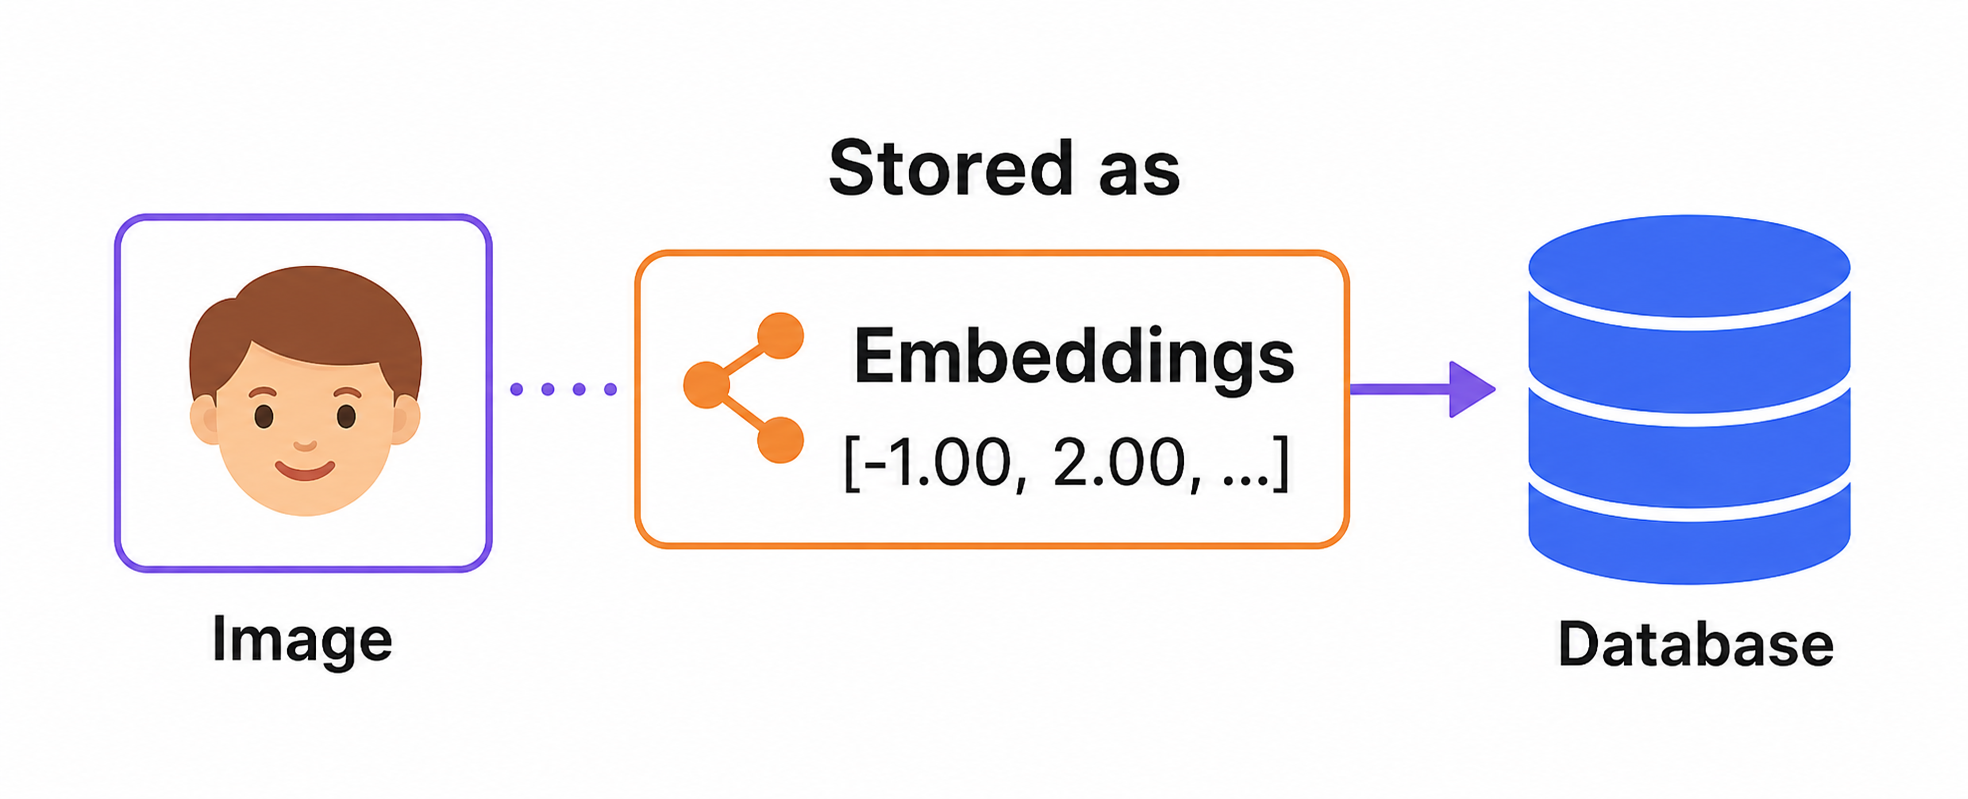
\includegraphics[width=0.62\textwidth]{embeddings.png}
\caption{Conceptual representation of embedding generation and vector storage adopted for facial identification within the proposed educational monitoring platform.}
\label{fig:embeddings}
\end{figure}
\FloatBarrier

Within educational monitoring contexts, embedding-based facial identification enables longitudinal classroom observation and temporal behavioral analytics while reducing unnecessary exposure of raw facial images. This strategy contributes to privacy-aware educational monitoring approaches but does not, by itself, establish legal or regulatory compliance.

After the embedding generation process, facial representations are projected into a high-dimensional vector space in which similar identities remain spatially close while distinct identities become mathematically separated \cite{schroffFaceNetUnifiedEmbedding2015,dengArcFaceAdditiveAngular}. This spatial organization enables the platform to compare identities through similarity metrics such as cosine distance and Euclidean distance \cite{nguyenCosineSimilarityMetric2011}.

The ability to distinguish different individuals within this vector space is one of the central characteristics responsible for the robustness of contemporary facial recognition architectures, particularly models based on ArcFace and InsightFace-related pipelines \cite{dengArcFaceAdditiveAngular,anKillingTwoBirds2022}.

Figure~\ref{fig:arcface_cnn} illustrates the conceptual process through which facial images are transformed into numerical vector representations capable of supporting similarity comparison and identity differentiation operations.

\begin{figure}[!htbp]
\centering
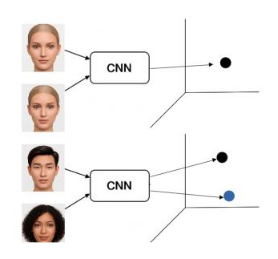
\includegraphics[width=0.50\textwidth,height=0.22\textheight,keepaspectratio]{arcface_cnn.png}
\caption{Conceptual representation of facial identity differentiation within high-dimensional embedding space generated through convolutional neural network architectures.}
\label{fig:arcface_cnn}
\end{figure}

Within the proposed platform, these vector representations are subsequently stored in PostgreSQL integrated with PGVector, enabling similarity retrieval and longitudinal educational monitoring operations \cite{zhangAreThereFundamental2024,panSurveyVectorDatabase2024}.
% TODO AUTOR: inserir referência técnica oficial sobre PGVector, caso exigida pela revista.


\subsection{Ethical and Privacy Considerations in Educational Monitoring}

The application of Artificial Intelligence and Computer Vision within educational environments raises important ethical and privacy-related concerns involving biometric processing, behavioral interpretation, and educational data governance.

Several studies emphasize that educational monitoring systems should avoid deterministic interpretation of student behavior or emotional states, particularly in scenarios involving automated inference mechanisms. Consequently, observational educational analytics should prioritize teacher support and contextual interpretation instead of disciplinary or psychological classification.

In this context, the present study adopts a privacy-aware architecture based on embedding representations instead of continuous raw facial image storage. Facial identification is performed through vector similarity search using normalized embeddings stored in PostgreSQL integrated with PGVector.

Additionally, the proposed platform was intentionally designed as a pedagogical support tool without diagnostic, psychological, or medical purposes. Behavioral indicators generated by the system are interpreted exclusively as observable classroom interaction patterns intended to support reflective pedagogical observation and Learning Analytics processes.


\section{Methodology}

This study adopted an applied technological research approach focused on the development of an intelligent platform for observational learning analytics in classroom environments. The experiments were conducted in a controlled laboratory environment designed to simulate classroom monitoring conditions using RTSP video streams.

\subsection{Platform Architecture}
The proposed architecture integrates real-time video acquisition, pose estimation, facial recognition, vector similarity search, behavioral inference, and temporal reporting modules. Figure~\ref{fig:architecture} presents the general workflow of the platform.

The workflow starts with the camera module, which provides the RTSP video stream used as the input for real-time classroom monitoring. The pre-processing stage then prepares the captured frames for inference by organizing the visual input before it is forwarded to the analytical modules. YOLOv11-Pose processes these frames to detect individuals and extract anatomical keypoints, which are used by the behavioral inference module to interpret observable posture, movement, and hand-raising patterns. In parallel, InsightFace processes detected facial regions to generate or compare facial embeddings, supporting the association between visual observations and previously registered students.

The PostgreSQL/PGVector layer stores structured monitoring records and vector representations, enabling similarity search between embeddings captured during monitoring and embeddings associated with registered students. Finally, the dashboard presents the resulting monitoring information and temporal analytics for pedagogical interpretation. In this architecture, pose estimation and facial recognition perform complementary functions: pose estimation supports behavioral interpretation, whereas facial recognition supports association with the registered student within the controlled experimental setting.

\begin{figure}[!htbp]
\centering
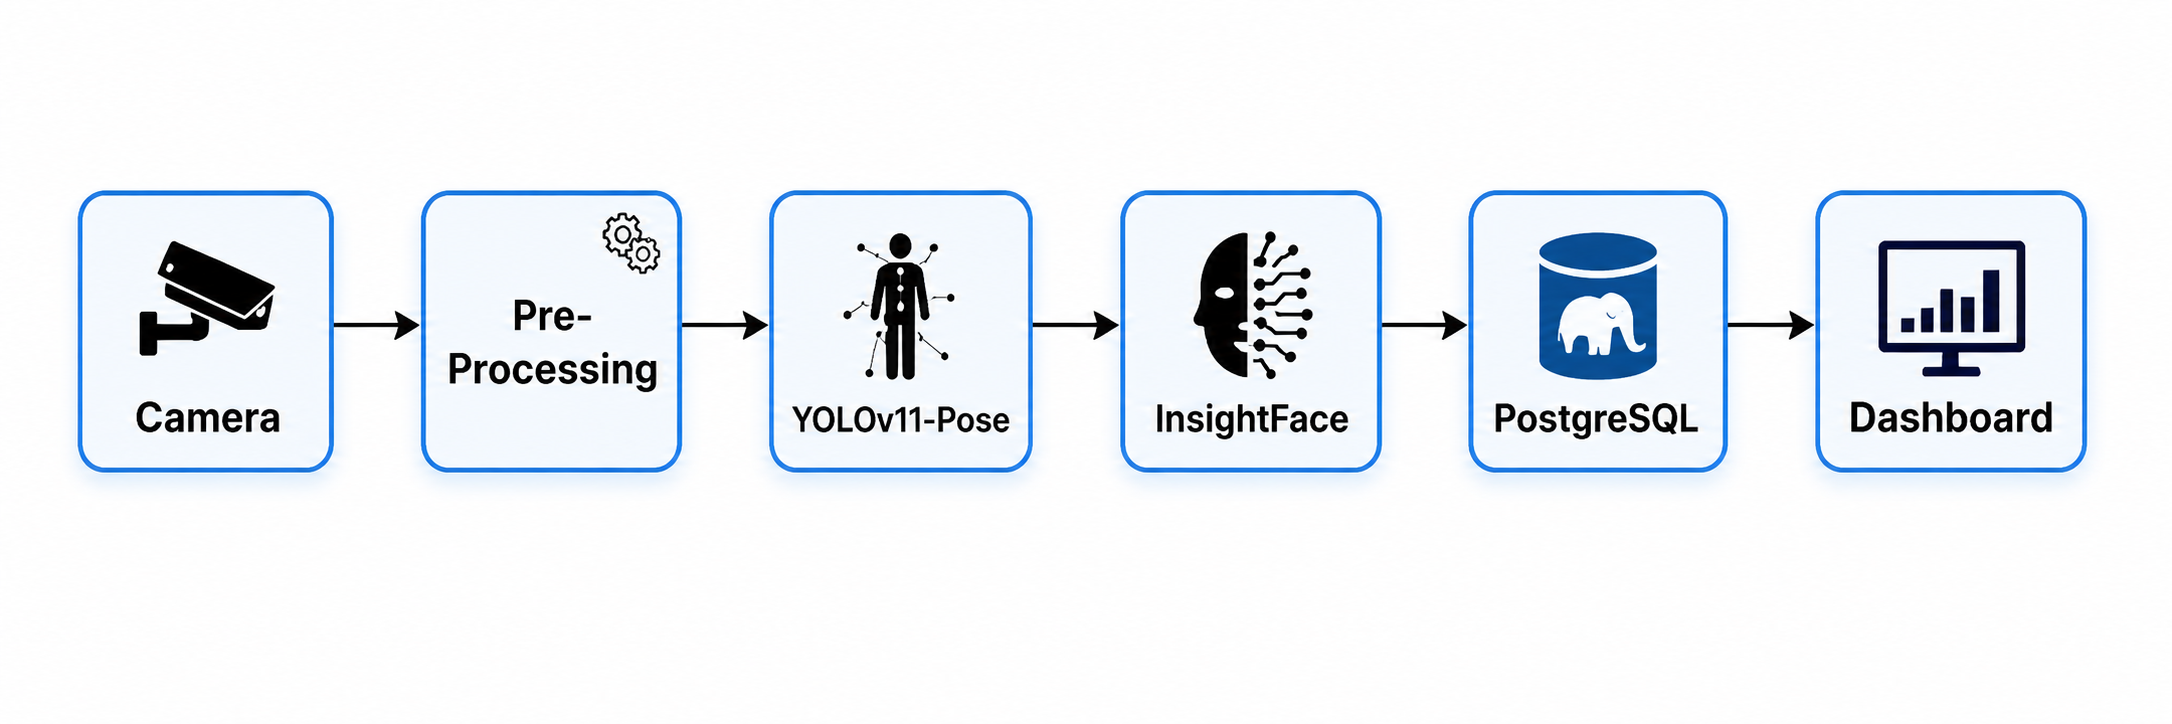
\includegraphics[width=0.95\textwidth]{architecture.png}
\caption{General architecture of the proposed observational learning analytics platform, showing the workflow from RTSP camera acquisition and frame pre-processing to YOLOv11-Pose estimation, InsightFace facial embedding processing, PostgreSQL/PGVector storage and similarity search, and dashboard-based temporal reporting.}
\label{fig:architecture}
\end{figure}

\subsection{Real-Time Pose Estimation}

The proposed platform employs YOLOv11-Pose to perform real-time human pose estimation from classroom video streams, following recent advances in real-time classroom behavior monitoring using YOLO-based architectures \cite{liangYOLObasedBehaviorDetection2025,zhuCsbyoloRapidEfficient2024}. Through this approach, the platform extracts anatomical keypoints associated with facial and upper-body structures, including the nose, eyes, shoulders, elbows, and wrists. These spatial references are subsequently used to support the geometric interpretation of observable classroom interaction patterns.

In the developed architecture, YOLOv11-Pose was adopted because it integrates object detection and human pose estimation within a single real-time inference pipeline. This characteristic reduces redundant processing steps by simultaneously detecting individuals and estimating their anatomical keypoints, which is particularly relevant in classroom environments containing multiple students in movement.

The model enables the extraction of structured spatial coordinates representing body regions such as the head, shoulders, elbows, and wrists. These keypoints are used as the computational basis for reconstructing upper-body posture and interpreting observable classroom interaction patterns. Therefore, YOLOv11-Pose supports continuous behavioral monitoring by transforming video frames into geometric representations suitable for real-time pedagogical analysis.

Rather than relying exclusively on facial analysis, the use of pose estimation enables the platform to capture broader postural and movement-related indicators associated with classroom participation dynamics. Figure~\ref{fig:pose} illustrates an example of the pose estimation process performed during classroom observation.

\begin{figure}[!htbp]
\centering
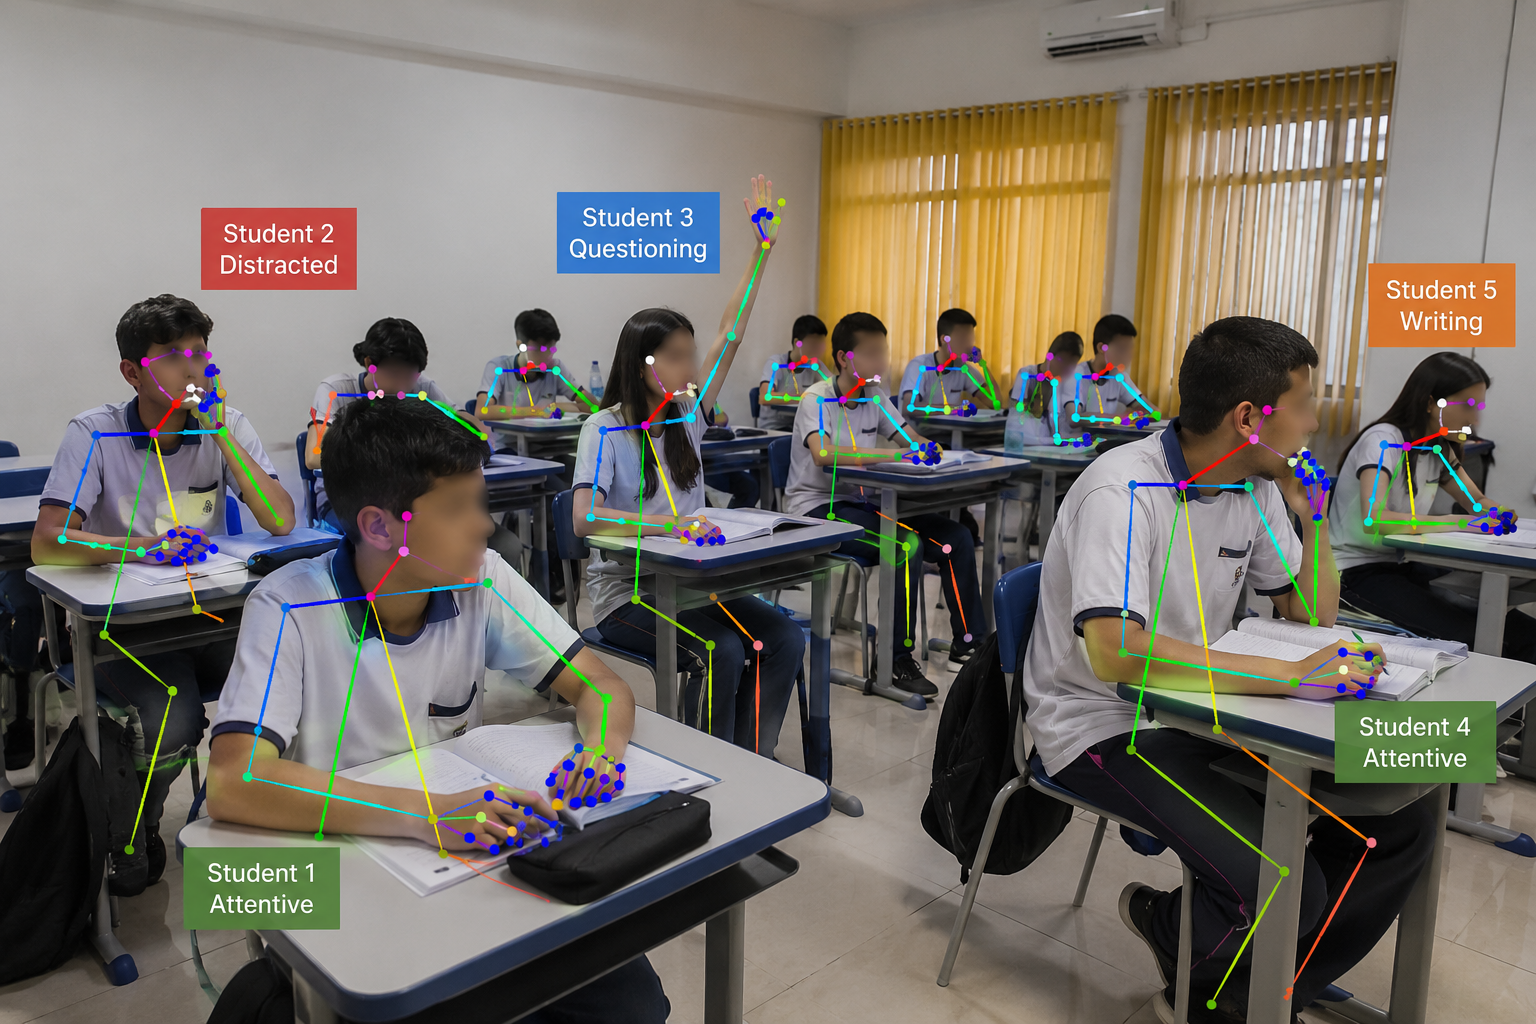
\includegraphics[width=0.75\textwidth]{pose_estimation.png}
\caption{Illustrative representation of classroom pose estimation and behavioral observation within the proposed educational behavioral analytics framework.}
% TODO AUTOR: confirmar autoria, origem e autorização de uso da imagem da Figura 5.
\label{fig:pose}
\end{figure}

Student identification is performed using InsightFace with ArcFace-based facial embeddings. During the registration process, facial images are converted into multidimensional numerical representations capable of preserving discriminative facial characteristics. The generated embeddings are stored in PostgreSQL integrated with PGVector, enabling vector similarity search through cosine distance comparison.

This strategy improves scalability while reducing the dependency on continuous raw image storage. In the proposed platform, facial recognition is used exclusively to associate observable behavioral records with previously registered students within the controlled educational environment.

Behavioral interpretation is based on geometric analysis of body keypoints extracted through pose estimation. Instead of relying on black-box emotional inference approaches, the system prioritizes interpretable classroom behavioral indicators that can support pedagogical observation.

The behavioral analysis module was designed to identify visible tendencies related to attentive posture, distraction patterns, agitation, prolonged downward head positioning, and hand-raising interactions commonly associated with questioning behavior. These categories are interpreted exclusively as observational indicators rather than definitive representations of cognitive, emotional, or psychological conditions. Figure~\ref{fig:behaviors} presents the behavioral interpretation framework adopted by the platform.

\FloatBarrier

\begin{figure}[!htbp]
\centering
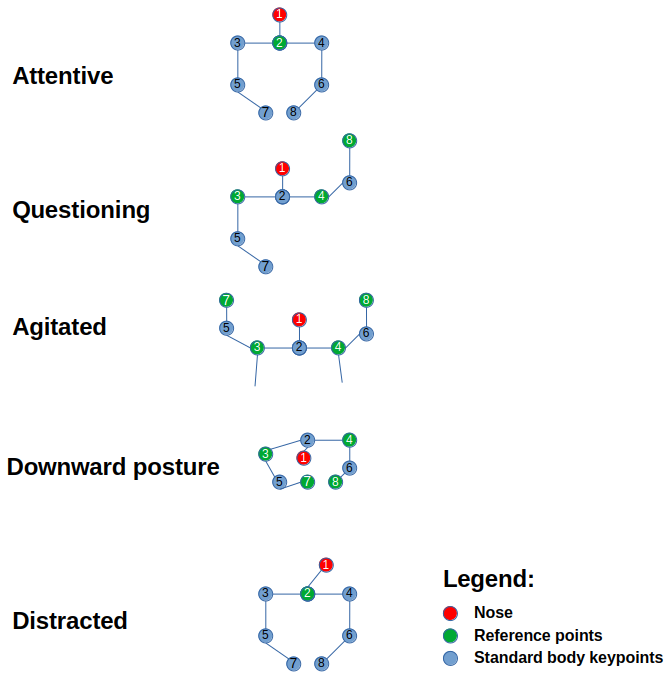
\includegraphics[height=0.35\textheight]{behaviors.png}
\caption{Behavioral interpretation framework adopted by the proposed platform for identifying observable classroom interaction patterns through geometric analysis of body keypoints estimated using YOLOv11-Pose.}
\label{fig:behaviors}
\end{figure}

\FloatBarrier

\subsubsection{Geometric Behavioral Interpretation}

The behavioral interpretation module adopted by the proposed platform was designed to prioritize interpretable geometric analysis instead of black-box emotional inference approaches, following recent ethical concerns involving affective educational AI systems \cite{xiaoOcclusionRobustCognitive2024,trabelsiRealTimeAttentionMonitoring2023a}. Observable classroom behaviors are inferred through spatial relationships among anatomical keypoints extracted using YOLOv11-Pose.

Rather than attempting psychological or affective classification, the system focuses exclusively on visible classroom interaction patterns associated with pedagogical observation and engagement monitoring.

The behavioral inference process is based on geometric relationships involving facial orientation, head inclination, wrist positioning, upper-body posture, and movement dynamics extracted from real-time classroom video streams \cite{yangStudentClassroomBehavior2024,chenStudentBehaviorDetection2023}.

To reduce isolated false-positive detections and improve temporal stability, the proposed platform applies short temporal consistency thresholds before confirming behavioral state transitions. Observable behaviors are validated only when the associated geometric conditions remain stable across consecutive frames for a minimum temporal interval.

This strategy reduces abrupt classification oscillations caused by temporary occlusions, natural body movement, lighting variation, or transient pose estimation instability during classroom monitoring sessions. Consequently, the platform prioritizes sustained observable interaction patterns rather than isolated instantaneous detections.

Table~\ref{tab:behavior_rules} summarizes the principal geometric interpretation criteria adopted by the proposed framework.

\begin{table}[htbp]
\centering
\caption{Geometric interpretation criteria adopted for observable classroom behavior analysis.}
\label{tab:behavior_rules}
\begin{tabularx}{\textwidth}{>{\raggedright\arraybackslash}p{2.8cm} Y Y}
\toprule
\textbf{Behavior} & \textbf{Geometric Criteria} & \textbf{Observational Interpretation} \\
\midrule

Attentive &
Stable head alignment and forward facial orientation with balanced upper-body posture &
Sustained classroom attention and instructional focus \\

Distracted &
Lateral head deviation or inconsistent facial orientation relative to the instructional direction &
Attention fluctuation or reduced engagement tendency \\

Questioning &
Wrist positioned above head level during instructional interaction &
Possible participation gesture or questioning-related interaction \\

Agitated &
Abrupt upper-body movement or excessive arm displacement across consecutive frames &
Elevated movement dynamics during classroom activities \\

Downward posture &
Head inclination below shoulder reference line for prolonged intervals &
Reduced alert posture or downward attention orientation \\

\bottomrule
\end{tabularx}
\end{table}

The proposed approach emphasizes explainable behavioral interpretation through observable geometric relationships instead of probabilistic emotional classification. This strategy contributes to greater interpretability, pedagogical transparency, and ethical compatibility within educational monitoring environments.

Additionally, facial identification is performed through cosine similarity comparison between normalized ArcFace embeddings stored in PostgreSQL integrated with PGVector. Cosine similarity was adopted because ArcFace embeddings are optimized for angular discrimination within normalized hyperspherical vector spaces, enabling efficient identity differentiation through vector similarity retrieval operations.


\FloatBarrier
\subsection{Experimental Environment}

The experimental validation of the proposed platform was conducted using a real-time processing environment configured for Computer Vision and Deep Learning inference tasks. Table~\ref{tab:environment} summarizes the main computational specifications adopted during the experiments.

The experimental validation was conducted as a proof-of-concept in a controlled laboratory environment using RTSP video streams to simulate classroom monitoring conditions. The processing workflow was configured to evaluate real-time pose estimation, facial association, behavioral interpretation, and temporal analytics under controlled observation conditions.

Before the monitoring sessions, participants were registered through a facial embedding workflow in which facial images were converted into normalized numerical representations and associated with registered identifiers for subsequent vector similarity retrieval. The controlled experimental setting was adopted to validate the technical feasibility of the proposed platform before future evaluation in real classroom environments, where factors such as illumination variation, occlusion, camera positioning, classroom density, and interaction dynamics may influence system performance.
% TODO AUTOR: informar número de participantes do experimento.
% TODO AUTOR: informar procedimento de consentimento/autorização.
% TODO AUTOR: descrever processo de cadastro facial dos voluntários.
% TODO AUTOR: informar local institucional ou caracterização do ambiente experimental.
% TODO AUTOR: informar posicionamento da câmera e condições de iluminação.

\begin{table}[htbp]
\centering
\caption{Processing environment specifications adopted during the experiments.}
\label{tab:environment}
\begin{tabularx}{\textwidth}{>{\raggedright\arraybackslash}p{4cm} Y}
\toprule
\textbf{Component} & \textbf{Specification} \\
\midrule
Operating System & Ubuntu 22.04 LTS \\

Primary GPU & NVIDIA RTX 3080 Ti -- 12 GB VRAM \\

Acceleration Frameworks & CUDA 12, cuDNN, TensorRT \\

Libraries and Frameworks & YOLOv11-Pose, InsightFace, Streamlit, PostgreSQL, PGVector \\

Video Acquisition & RTSP IP Camera (Hikvision 2 MP) \\
\bottomrule
\end{tabularx}
\end{table}

CUDA Toolkit, cuDNN, and TensorRT were employed to optimize GPU-based inference operations, reducing latency and improving real-time processing efficiency during behavioral monitoring tasks. The experiments demonstrated that the proposed platform can operate efficiently using a single intermediate-class GPU, reinforcing its feasibility for educational deployment scenarios.

\subsection{Facial Recognition and Vector Similarity Workflow}

The proposed platform performs student identification through an embedding-based facial recognition architecture integrating InsightFace, ArcFace representations, PostgreSQL, and PGVector vector retrieval operations \cite{dengArcFaceAdditiveAngular,schroffFaceNetUnifiedEmbedding2015,anKillingTwoBirds2022}. During classroom monitoring activities, facial regions are continuously detected from RTSP video streams and converted into normalized numerical embeddings optimized for similarity comparison through cosine-based vector retrieval mechanisms \cite{nguyenCosineSimilarityMetric2011}.

Unlike traditional image-based storage approaches, the proposed framework prioritizes vector representations capable of preserving discriminative facial characteristics while reducing dependency on continuous raw biometric image retention. This strategy contributes to real-time identification efficiency while supporting privacy-aware educational monitoring practices, although additional institutional, legal, and governance procedures remain necessary for any operational deployment.

Figure~\ref{fig:facial_pipeline} presents the complete facial recognition and vector similarity workflow adopted by the proposed educational monitoring platform.

\FloatBarrier
\begin{figure}[htbp]
\centering
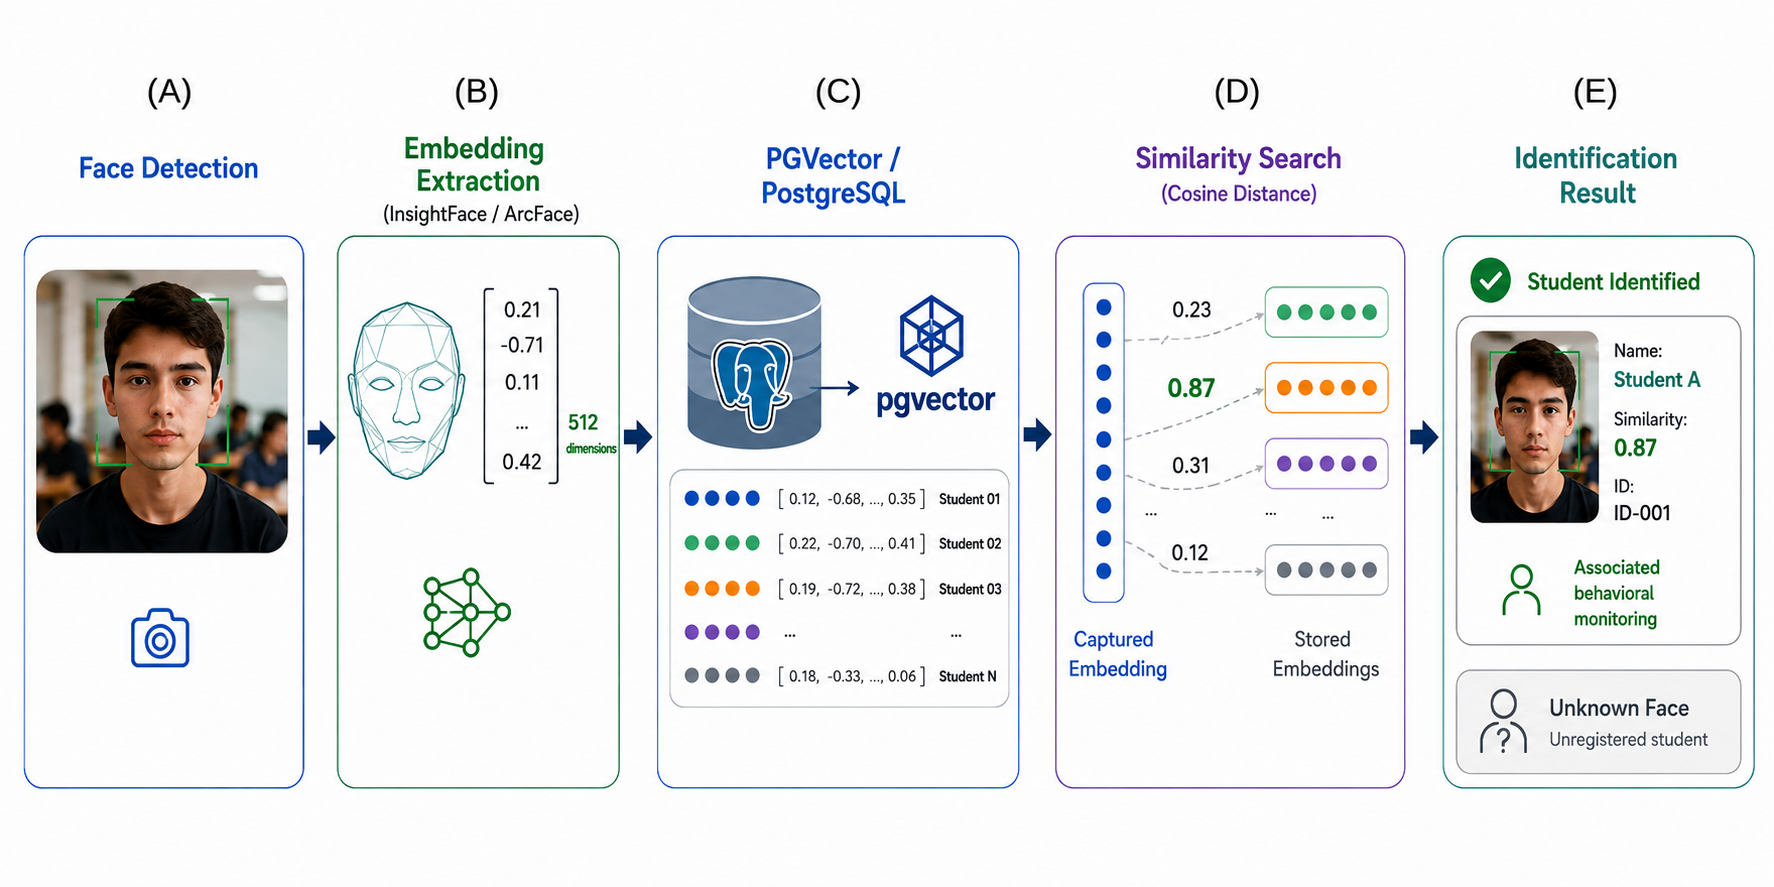
\includegraphics[width=0.98\textwidth]{facial_pipeline.png}
\caption{Facial recognition and vector similarity retrieval workflow integrating InsightFace, ArcFace embeddings, PostgreSQL, and PGVector for real-time educational monitoring.}
\label{fig:facial_pipeline}
\end{figure}
\FloatBarrier

Recent advances in embedding-based facial recognition have demonstrated high discriminative capability for real-time identity retrieval tasks in unconstrained environments \cite{dengRetinaFaceSinglestageDense2019,schroffFaceNetUnifiedEmbedding2015}.

The workflow illustrated in Figure~\ref{fig:facial_pipeline} is composed of five integrated stages responsible for transforming classroom video streams into identifiable educational monitoring information.

In stage \textbf{(A)}, facial regions are continuously detected from RTSP classroom video streams using InsightFace-based detection mechanisms. This initial step allows the platform to isolate visible student faces from the classroom scene in real time, even in environments containing multiple individuals simultaneously positioned within the camera field of view.

In stage \textbf{(B)}, each detected facial region is processed to generate a normalized 512-dimensional embedding using ArcFace-based representations \cite{dengArcFaceAdditiveAngular} implemented through InsightFace. Instead of storing the original facial image itself, the system converts the facial characteristics into a compact numerical vector capable of preserving discriminative identity information while reducing dependency on continuous raw biometric image storage.

In stage \textbf{(C)}, the generated embeddings are stored within PostgreSQL integrated with the PGVector extension. This vector-based storage architecture enables efficient indexing and retrieval operations specifically optimized for high-dimensional similarity comparison tasks. The use of PGVector allows the platform to maintain scalable facial representation repositories compatible with real-time educational monitoring scenarios.

Subsequently, stage \textbf{(D)} performs cosine similarity comparison between the embedding captured during classroom monitoring and the embeddings previously registered within the vector database, enabling angular similarity retrieval through high-dimensional vector comparison \cite{nguyenCosineSimilarityMetric2011}. During this process, the system searches for the closest vector representation according to angular similarity distance, enabling identification through mathematical comparison rather than direct image matching.

Cosine similarity measures the angular proximity between normalized embeddings represented within hyperspherical vector spaces. In this approach, embeddings associated with the same individual tend to present smaller angular distances and higher cosine similarity values, while embeddings belonging to different individuals remain spatially separated within the vector space.

This strategy is particularly compatible with ArcFace-based representations \cite{dengArcFaceAdditiveAngular} because ArcFace optimizes embedding discrimination through additive angular margin learning. Consequently, cosine similarity enables robust identity differentiation while reducing sensitivity to embedding magnitude variations, favoring efficient vector retrieval operations during real-time educational monitoring.

Finally, in stage \textbf{(E)}, the platform retrieves the most similar registered embedding and associates the identified student with the corresponding behavioral monitoring analytics generated during classroom observation activities. This integration enables simultaneous facial recognition, behavioral interpretation, and longitudinal educational monitoring within a unified real-time analytical environment.

\section{Results and discussion}

The proposed platform successfully integrated real-time video acquisition, pose estimation, facial recognition, vector similarity search, and behavioral analytics into a unified educational monitoring environment, similarly to recent intelligent classroom monitoring proposals reported in the literature \cite{mitomaBehaviorMonitoringSystem2025,huRealTimeClassroomBehavior2024}. During the experiments conducted in a controlled laboratory classroom scenario, the system was capable of identifying observable classroom interaction patterns in real time through geometric analysis of body keypoints extracted using YOLOv11-Pose.

The integration between InsightFace and PGVector enabled individual student association through vector similarity search using facial embeddings generated with ArcFace-based representations \cite{dengArcFaceAdditiveAngular}. This approach allowed the platform to associate behavioral observations with previously registered students while reducing the dependency on continuous raw image storage.

\subsection{Real-Time Behavioral Monitoring}
Figure~\ref{fig:realtime} presents an example of real-time classroom monitoring performed by the proposed platform during instructional activities. The platform simultaneously performs pose estimation, student identification, and observational behavioral interpretation in real time.

\FloatBarrier
\begin{figure}[htbp]
\centering
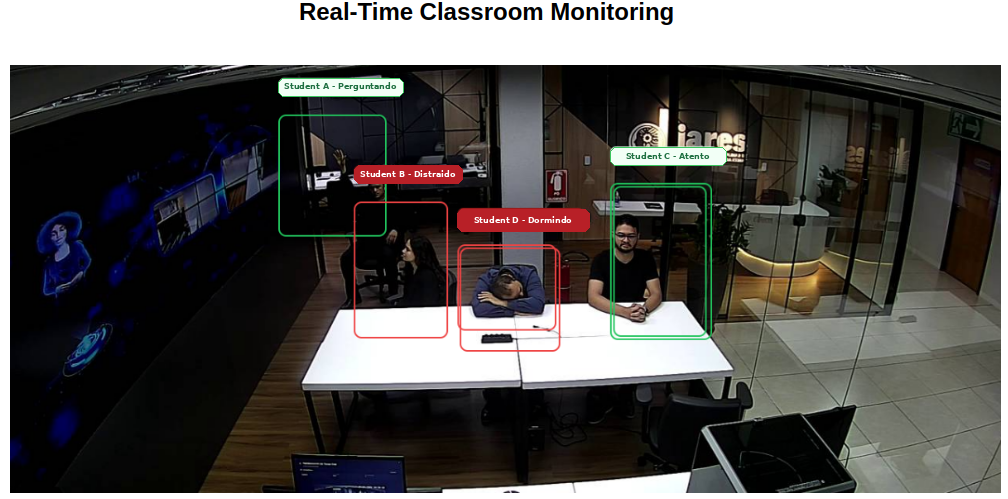
\includegraphics[width=0.95\textwidth]{figure8_blinded.png}
\caption{Real-time monitoring dashboard demonstrating simultaneous multi-subject identification and behavioral classification. Behavioral labels displayed in Portuguese correspond to the classroom states ``Questioning'', ``Distracted'', ``Downward posture'', and ``Attentive''. Identifiers displayed in the monitoring interface were anonymized for double-blind review.}
\label{fig:realtime}
\end{figure}
\FloatBarrier


The experimental results demonstrated that the proposed framework was capable of identifying observable classroom interaction tendencies associated with attentive posture, distraction patterns, agitation, downward head positioning, and questioning-related gestures during monitoring sessions. Rather than attempting emotional recognition or psychological inference, the proposed approach prioritizes interpretable observational indicators intended to support pedagogical reflection and classroom engagement analysis.

One of the central contributions of the proposed platform involves the generation of temporal behavioral analytics intended to support reflective pedagogical observation and educational management. Instead of emphasizing isolated behavioral events, the system enables longitudinal analysis of classroom interaction dynamics throughout instructional periods.

\subsection{Temporal Behavioral Analytics}

The behavioral distribution analytics presented in Figure~\ref{fig:pizza} provide a macro-level overview of the predominant classroom interaction patterns observed during instructional activities. This type of visualization may assist educators in identifying engagement tendencies, distraction prevalence, participation dynamics, and broader classroom behavioral profiles during instructional sessions.

\FloatBarrier
\begin{figure}[htbp]
\centering
\vspace{-0.2cm}
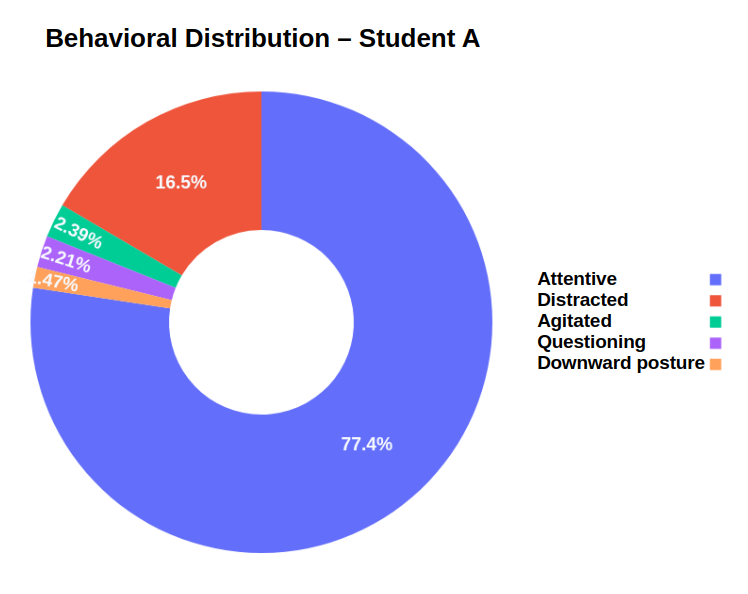
\includegraphics[width=0.70\textwidth]{graphic_pizza.png}
\vspace{-0.3cm}
\caption{Behavioral distribution generated by the proposed platform presenting the percentage of time associated with each observed classroom behavior during instructional activities.}
\label{fig:pizza}
\vspace{-0.2cm}
\end{figure}
\FloatBarrier


Beyond global behavioral distribution, the proposed platform also enables temporal analysis of behavioral evolution throughout classroom sessions. Figure~\ref{fig:timeline} illustrates how classroom behaviors fluctuate during instructional periods, enabling the identification of concentration intervals, interaction moments, distraction peaks, and engagement variability over time.

This temporal perspective is particularly relevant for pedagogical management because classroom behavior naturally changes according to instructional methodology, classroom dynamics, and activity type. Consequently, short moments of distraction or movement should not necessarily be interpreted as negative indicators, but rather as components of ordinary classroom interaction processes. In this context, temporal behavioral analytics may support reflective teaching practices, instructional adaptation strategies, and broader learning analytics initiatives focused on classroom engagement observation.

\FloatBarrier
\begin{figure}[htbp]
\centering
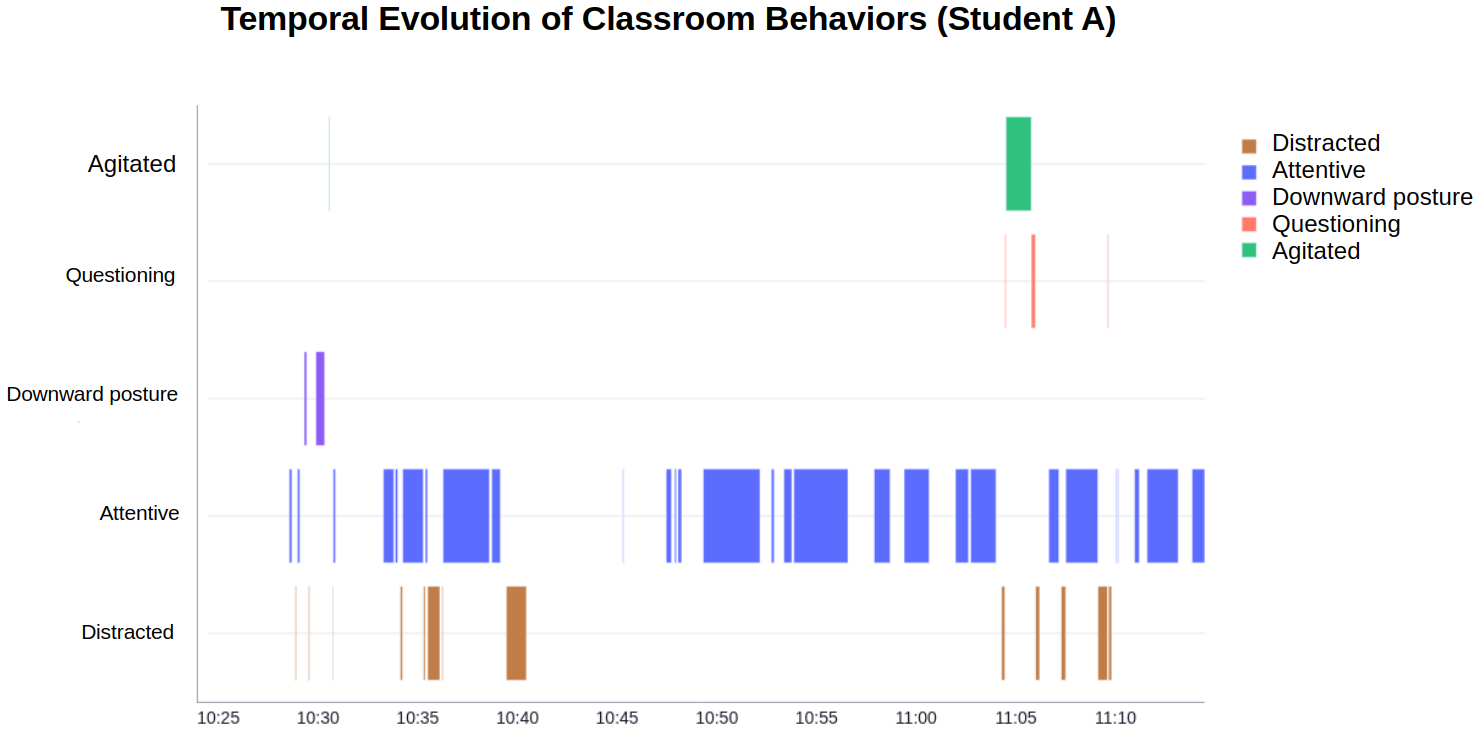
\includegraphics[width=1.0\textwidth]{graphic_temporal.png}
\caption{Temporal evolution of observed classroom behaviors throughout instructional periods, enabling longitudinal analysis of engagement tendencies and classroom interaction dynamics.}
\label{fig:timeline}
\end{figure}
\FloatBarrier

\subsection{Comparative Instructional Context Analysis}

In addition to individual behavioral distribution and temporal evolution analysis, the proposed platform also enables comparative behavioral observation across different instructional contexts. This capability is particularly relevant for pedagogical management because classroom interaction patterns may vary according to teaching methodology, instructional strategy, and activity type.

Figure~\ref{fig:graphic_type} presents a comparative behavioral analysis between distinct instructional contexts monitored by the proposed platform. The generated analytics allow educators to observe how engagement tendencies, distraction levels, questioning behavior, and movement dynamics fluctuate according to classroom activity characteristics.

Such comparative visualization may support reflective teaching practices by enabling broader interpretation of classroom engagement dynamics throughout different pedagogical scenarios. Rather than evaluating isolated student actions, the proposed approach prioritizes contextual and longitudinal observation capable of assisting teachers in understanding how instructional environments may influence classroom interaction patterns.

\FloatBarrier
\begin{figure}[htbp]
\centering
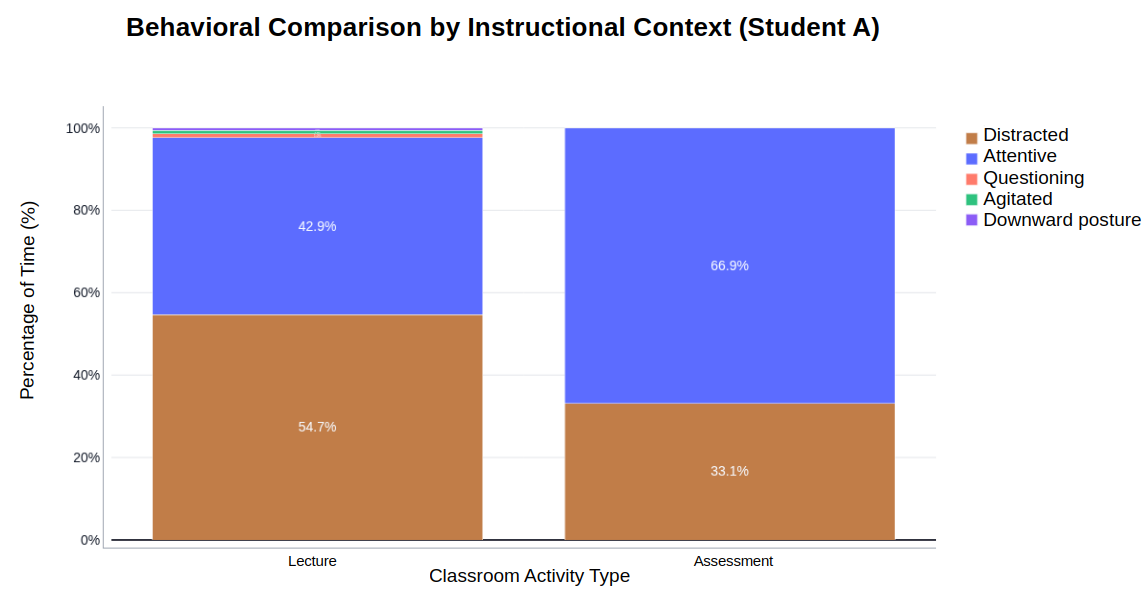
\includegraphics[width=0.88\textwidth]{graphic_type.png}
\caption{Comparative behavioral analysis across different instructional contexts generated by the proposed platform, enabling observation of engagement and interaction tendencies according to classroom activity type.}
\label{fig:graphic_type}
\end{figure}
\FloatBarrier

\subsection{Longitudinal Observational Synthesis and Case Study}

The platform's ability to generate longitudinal observational summaries was validated through a case study involving a 54.4-minute instructional session. The system processed the continuous video stream to correlate individual behavioral events into a pedagogically meaningful report.

\subsubsection{Quantitative Behavioral Profile}

Table~\ref{tab:behavioral_results} presents the definitive behavioral distribution for the monitored subject (Student A). The data indicates a high level of engagement, with the "Attentive" state persisting for 77.3\% of the total session time (42.1 minutes).

\begin{table}[!htbp]
\centering
\caption{Quantitative distribution of observed classroom behaviors for Student A.}
\label{tab:behavioral_results}
\begin{tabularx}{\textwidth}{@{}>{\raggedright\arraybackslash}p{3.8cm} c c Y@{}}
\toprule
\textbf{Behavior Category} & \textbf{Accumulated Time} & \textbf{Percentage (\%)} & \textbf{Frequency Status} \\ \midrule
Attentive (Atento)         & 42.1 min                 & 77.3\%                  & Predominant               \\
Distracted (Distraído)     & 9.0 min                  & 16.6\%                  & Occasional                \\
Agitated (Agitado)         & 1.3 min                  & 2.4\%                   & Low Frequency             \\
Questioning (Perguntando)  & 1.2 min                  & 2.1\%                   & Low Frequency             \\
Downward posture (prototype label: `Dormindo')      & 0.8 min                  & 1.5\%                   & Low Frequency             \\ \bottomrule
\end{tabularx}
\end{table}

The temporal behavioral distribution presented in Figure~\ref{fig:timeline_distribution} provides additional evidence regarding the concentration of behavioral fluctuations throughout the instructional session. The generated analytics indicate that most non-attentive behavioral occurrences associated with Student A were concentrated during the initial phase of the class, while the middle and final instructional periods demonstrated greater behavioral stability and sustained attentive posture.

From a pedagogical perspective, this type of temporal distribution analysis may assist educators in identifying specific instructional moments associated with reduced engagement or adaptation difficulty. In the observed session, the concentration of distracted and agitated behaviors during the beginning of the class may suggest transitional adaptation effects related to the initial instructional context, environmental adjustment, or early classroom interaction dynamics.

Such temporal insights reinforce the importance of longitudinal classroom observation rather than isolated behavioral interpretation. Instead of characterizing individual behaviors as definitive indicators, the proposed platform prioritizes contextual analytics capable of supporting reflective pedagogical practices and broader learning analytics strategies focused on classroom engagement monitoring.

\FloatBarrier
\begin{figure}[htbp]
\centering
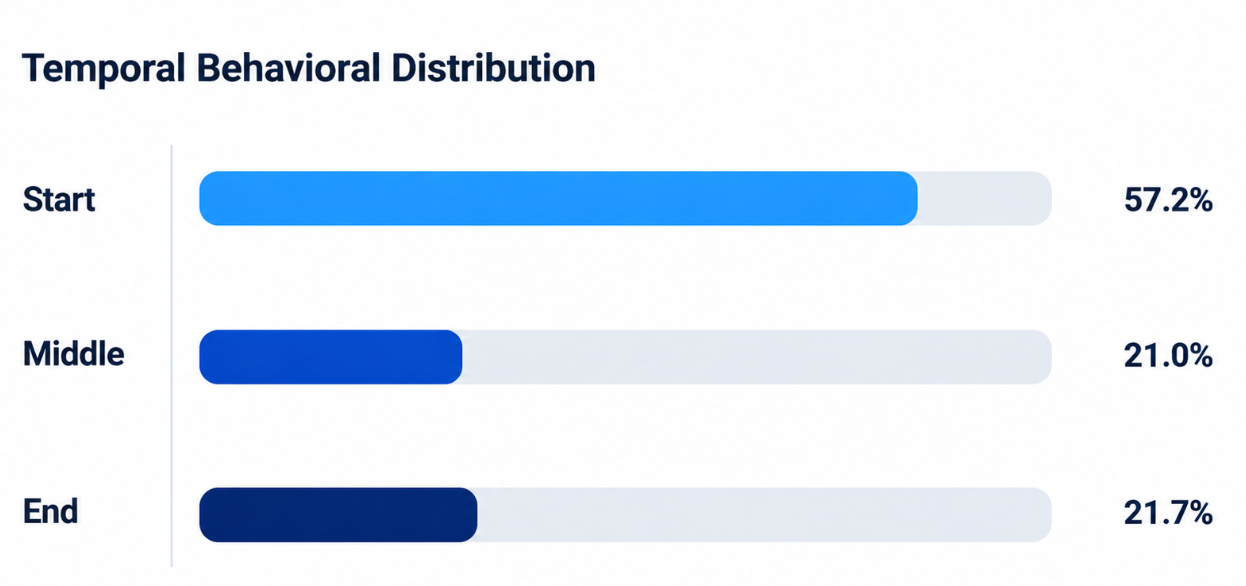
\includegraphics[width=0.78\textwidth]{temporal_behavioral_distribution.png}
\caption{Temporal behavioral distribution generated by the proposed platform presenting the concentration of observed classroom behaviors throughout the beginning, middle, and final instructional periods for Student A.}
\label{fig:timeline_distribution}
\end{figure}
\FloatBarrier

\subsubsection{Temporal Dynamics and Pedagogical Insights}

Beyond simple quantification, the platform identified significant temporal fluctuations in engagement. A concentration of "Distracted" (16.6\%) and "Agitated" (2.4\%) behaviors was detected specifically during the initial phase of the lesson. From an instructional design perspective, this peak suggests that the transition into the activity or the initial instructional delivery may have encountered environmental or cognitive barriers that reduced student focus.

Conversely, the "Questioning" behavior (2.1\%), characterized by specific hand-raising keypoint configurations, occurred in a distributed manner, indicating periods of active participation despite the initial distraction peaks. The minimal presence of "Downward posture" (1.5\%) suggests that the student maintained adequate physical alertness throughout the session.

\subsubsection{Decision Support and Recommendations}
The synthesized output provides actionable insights for pedagogical intervention. Based on the automated analysis, the platform recommended a "light follow-up" (light pedagogical follow-up), focusing on strategies to mitigate initial distraction. The system's ability to contrast current data with baseline expectations (or future sessions) demonstrates its potential for longitudinal pedagogical monitoring.


\subsubsection{Methodological and Ethical Limitations}
It is critical to note that the generated report functions as an observational support tool, not a clinical diagnostic mechanism. The estimated accumulated times are subject to environmental constraints such as camera framing, lighting variations, and physical occlusions in the classroom. Furthermore, privacy was maintained through the use of facial embeddings (ArcFace-based), ensuring that identification for the report (Cosine Similarity $\approx 0.83$) was performed without the persistent storage of raw biometric images, aligning with standard data protection guidelines for educational settings.



Recent studies have demonstrated the applicability of AI-based classroom monitoring systems for supporting behavioral interpretation, educational observation, and temporal learning analytics within intelligent educational environments. \cite{chenStudentBehaviorDetection2023,huRealTimeClassroomBehavior2024,liRealTimeClassroomBehavior2025,mitomaBehaviorMonitoringSystem2025,yangStudentClassroomBehavior2024}.

\section{Conclusion}

This study presented an intelligent behavioral monitoring platform designed to support observational learning analytics in basic education through the integration of Computer Vision, Artificial Intelligence, and temporal behavioral analytics. The proposed framework successfully combined YOLOv11-Pose for real-time pose estimation, InsightFace with ArcFace embeddings for facial identification, and PostgreSQL integrated with PGVector for vector similarity retrieval within a unified educational monitoring environment.

Unlike approaches centered on emotional inference or automated psychological classification, the proposed system was intentionally designed as a pedagogical support tool focused exclusively on observable classroom interaction patterns. Behavioral indicators were inferred through interpretable geometric relationships extracted from body keypoints, enabling explainable observational analytics compatible with reflective pedagogical practices.

The experimental results demonstrated the feasibility of performing simultaneous multi-subject monitoring, behavioral interpretation, temporal behavioral analytics, and embedding-based student association in real time. In addition, the generated longitudinal reports and temporal distribution analytics demonstrated potential for supporting classroom engagement analysis, instructional reflection, and educational decision-making processes.

From an ethical and privacy-oriented perspective, the proposed architecture contributes to educational monitoring approaches that minimize dependency on continuous raw biometric image storage by prioritizing normalized embedding representations and vector similarity retrieval operations. This strategy may reduce unnecessary exposure of raw facial images, although it does not replace formal data protection, consent, and governance procedures required in educational contexts.

Despite the promising results, the study presents important limitations. The experiments were conducted in a controlled laboratory environment involving proof-of-concept validation conditions, which may not fully represent the complexity of real classroom scenarios. Environmental factors such as illumination variation, physical occlusions, camera positioning, and classroom overcrowding may influence behavioral inference performance and monitoring stability.

Future work may investigate longitudinal deployments in real educational environments, teacher-centered validation methodologies, explainable behavioral analytics, adaptive temporal inference strategies, and additional privacy-preserving mechanisms for educational Artificial Intelligence systems. Furthermore, future studies may explore the integration of pedagogical dashboards capable of assisting teachers in interpreting behavioral tendencies throughout extended instructional periods.

Overall, the proposed platform contributes to the interdisciplinary intersection between Artificial Intelligence in Education, Learning Analytics, Computer Vision, and Intelligent Educational Systems by presenting an ethically oriented and pedagogically interpretable framework for real-time classroom behavioral observation.

\section*{Ethical Statement}

The proposed platform was developed exclusively for educational research and observational learning analytics purposes within a controlled laboratory environment. The system was not designed for psychological, medical, disciplinary, or biometric surveillance applications.

All demonstrations presented in this study were conducted using authorized research volunteers under controlled experimental conditions. The platform prioritizes privacy-aware processing through embedding-based facial representations rather than continuous raw biometric image storage.

Behavioral indicators generated by the system are interpreted exclusively as observable classroom interaction patterns intended to support reflective pedagogical analysis. No emotional inference, psychological profiling, or automated diagnostic decision-making is performed by the proposed framework. \cite{zhangClassroomBehaviorDetection2025,ClassroomBehaviorRecognition2025,hossenAttentionMonitoringStudents2023}.


\bibliographystyle{sn-mathphys-num}
\bibliography{references}

\end{document}
